\chapter*{Conclusion}
\addstarredchapter{Conclusion} 

Cette thèse est consacrée à la modélisation, à l'étude et au contrôle d'un drone convertible sujet à des forces aérodynamiques, des couplages entre les actionneurs et des dynamiques non-linéaires. Elle propose, au travers de l'utilisation d'un modèle unifié représentant les forces aérodynamiques sur l'ensemble du domaine de vol, d'analyser le comportement d'un \textit{tailsitter} et de proposer des méthodes de commande. Notre travail à débouché sur la proposition d'une nouvelle architecture de type \textit{freewing}.

La première partie du manuscrit propose un rapide aperçu des architectures de drone convertible avant de se focaliser sur les \textit{tailsitter} et les \textit{freewing}. Nous avons développé les principales caractéristiques d'actionnement, le comportement des drones ainsi que les méthodes de modélisation. Ce chapitre introductif a permis de développer l'architecture conventionnelle de commande, ainsi qu'un tour d'horizon des méthodes de commande et d'optimisation des contrôleurs. Notre travail ayant une forte composante expérimentale, une vision de l'architecture nécessaire à ces expérimentations a été évoquée avant d'être développée plus en profondeur dans l'annexe \ref{chap:annexe1}.  

Nous avons utilisé un modèle de la littérature, sans singularité sur l'ensemble du domaine de vol, ne faisant pas appel aux angles aérodynamiques $\alpha$ et $\beta$, appelé $\phi$-théorie. Ce modèle mathématique n'a d'utilité pratique que s'il est cohérent avec la réalité, ce qui a pu être démontré dans la littérature et qui est confirmé par nos travaux. De ce modèle non-linéaire, nous avons pu extraire des caractéristiques intéressantes pour les drones à décollage et atterrissage vertical. 
Nous avons caractérisé l'ensemble des points d'équilibre avec ou sans vent pour un \textit{tailsitter}. De ces équilibres, nous avons extrait la dynamique linéarisée, point de départ de la conception de toute loi de commande linéaire. Notre compréhension du comportement du drone a été augmenté par ces résultats qui nous informent sur la commandabilité du drone, sur les marges vis-à-vis des saturations et sur la capture du comportement du drone par une linéarisation autour des points d'équilibre. Nous avons donc pu valider la précision des linéarisations face aux nombreuses non-linéarités du modèle. Pour cela, nous avons effectué des simulations en boucle fermée, au vu du comportement instable du drone, du modèle linéaire et non-linéaire.

Un travail préliminaire a permis de proposer une architecture de commande hybride avec un mécanisme d'hystérésis, basée sur une variable discrète sélectionnant la loi de commande la plus appropriée en fonction de la phase de vol. Les deux lois proposées dans ce cas sont une loi non-linéaire basée sur une direction de zéro-moment et une loi linéaire LQR. Cette loi LQR est optimisée grâce au modèle obtenu précédemment.

De ce travail et à l'aide de la linéarisation, nous avons observé un comportement intéressant pour le rejet de perturbations de vent sur un \textit{tailsitter}. Ce comportement repose sur le changement de l'angle de tangage du drone pour compenser l'augmentation de la vitesse air qui engendre un déplacement du drone. Nous avons donc expérimenté, à l'aide d'une maquette à trois degrés de liberté, une loi de commande proportionnelle intégrale. Cette maquette, utilisant une architecture physique associée à un modèle de dynamique transactionnelle simulée, a permis de valider l'architecture de commande ainsi que son optimisation basée sur des contraintes $H_{\infty}$.
Bien que les résultats obtenus soient prometteurs, nous avons étudié une méthode différente d'obtention des gains du contrôleur PI. Cette méthode, plus conservative, est basée sur une résolution successive de LMI. Les résultats ont pu être évalués sur l'architecture complète du drone, par un vol expérimental en volière.

Cette expérimentation a permis d'identifier des problèmes de sensibilité de la boucle fermée aux dynamiques non modélisées et aux bruits. Nous avons donc proposé une extension du contrôleur PI pour augmenter sa robustesse. Une expérimentation face à un vent croissant par palier à validé notre travail.

Nos travaux nous ont amené à vouloir installer un capteur de vent sur le drone pour pouvoir utiliser la mesure pour la transition. Toutefois, le corps du \textit{tailsitter} étant en rotation lors de la transition, nous ne pouvions pas fixer le capteur de manière satisfaisante. Nous avons donc étudié et développé une architecture \textit{freewing} procurant un fuselage maintenu horizontal permettant d'installer n'importe quel capteur ou charge utile. L'aile étant en rotation libre autour du fuselage, nous conservons de nombreuses propriétés des \textit{tailsitters}. Dans cette démarche, nous avons modélisé le drone avec une dynamique multicorps, identifié les paramètres, fabriqué la maquette et réalisé des vols expérimentaux à l'aide de l'INDI.

\section*{Limite de l'étude}
Les travaux préliminaires, menés au chapitre \ref{chap:hybrid}, ne sont que des résultats de simulation. Il serait souhaitable de réaliser des expérimentations du contrôleur non-linéaire basé sur une direction de zéro-moment ainsi que de son utilisation dans l'architecture hybride avec une transition entre le contrôleur basé sur une direction de zéro-moment et le contrôleur PI étendu développé au chapitre \ref{chap:6DOF}.

Bien que nous souhaitions utiliser la mesure du vent, notre travail n'a pu aboutir par la richesse des questions que nous avons souhaité développer en amont et par le temps nécessaire au développement de l'architecture nécessaire.
De plus, de nombreuses architectures auraient pu répondre au besoin. Nous avons choisi de nous concentrer sur une architecture inspirée du \textit{tailsitter} DarkO car nous avions de l'expérience dans sa modélisation et sa dynamique.

Tous nos résultats ont été expérimentés dans une atmosphère contrôlée avec un générateur de perturbation. Il serait maintenant intéressant d'évaluer la précision de nos contrôleurs en extérieur. Ce travail possède une double complexité car le drone évoluerait dans un environnement plus turbulent, mais aussi avec une estimation d'état moins précise. Effectivement, en intérieur, nous avons accès à un système de positionnement millimétrique alors qu'en extérieur, les GPS ne peuvent nous fournir une information de position aussi précise.


\section*{Travaux futurs}
{
    \color{green}
La modélisation de Udwadia-Kalaba permet d'obtenir un modèle d'un drone multicorps. Il serait intéressant d'utiliser ces travaux pour concevoir un contrôleur assurant la stabilisation de l'aile et du fuselage en prenant en compte leurs interactions.

De plus ce contrôleur pourrait profiter de la mesure du vent réalisé par une sonde cinq trous installée sur le fuselage. Comme le fuselage est maintenu horizontal et avec une faible variation d'incidence, la mesure sera disponible dans toutes les phases de vol. Il est nécessaire de caractérisé la sonde. Effectivement, la mesure est réalisée par une différence de pression statique et dynamique, nous devons donc étudier la sensibilité des capteurs pour déterminer la plus petite variation de vent mesurable ainsi que le temps nécessaire à la mesure.

Enfin, nous terminerons la description des perspectives par un point qui reste sans réponse à ce jour. Ce point est relatif au guidage d'un drone convertible. Étant donné qu'ils possèdent deux modes de déplacement (stationnaire et vol d'avancement), quelle stratégie de vol adopté en fonction des caractéristiques de la mission ?
Autrement dit, étant donné un drone convertible en un point de l'espace, il est nécessaire de le faire rejoindre un autre point. En fonction de la distance entre les deux points, il faut choisir entre effectuer une transition du mode stationnaire vers le mode d'avancement (plus efficace énergétiquement) ou bien resté en stationnaire et se déplacer de proche en proche (très énergivore). Les contraintes sont multiples car bien que le vol d'avancement soit intéressant énergétiquement, il va nécessite deux transitions et pour un déplacement de courte distance, il nécessitera peut-être de réalisé un cercle pour avoir assez de temps de vol pour réaliser ces transitions. Ce problème est schématisé sur la Figure \ref{fig:pbhybride}.

\begin{figure}[ht!]
    \centerline{
    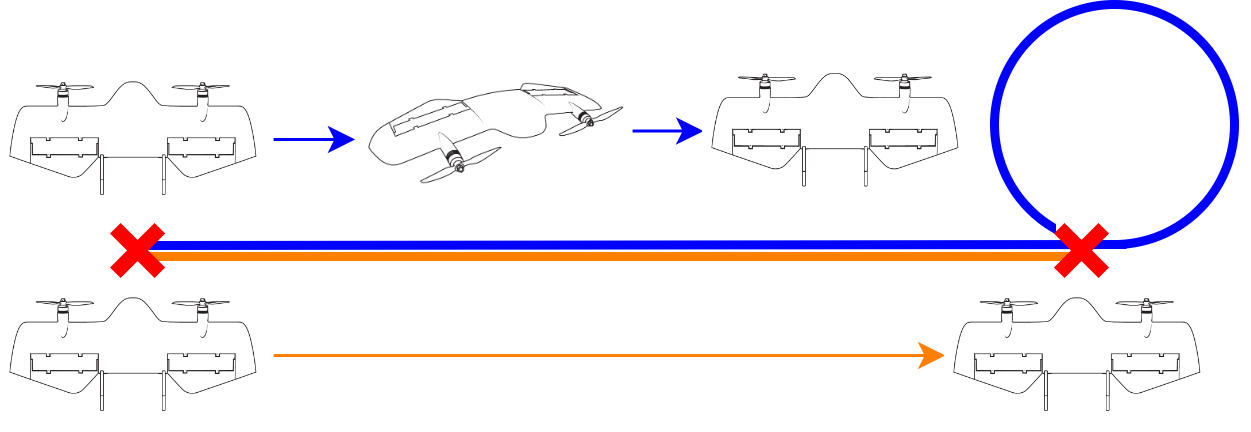
\includegraphics[trim=0cm 0cm 0cm 0cm,clip,width=0.8\columnwidth]{figures/DroneConvertibleGuidage.png}}
    \caption{Schéma de déplacement d'un drone convertible.}
    \label{fig:pbhybride}
\end{figure}


}
